\documentclass[12pt]{article}

%%%%%%%%%%%%%%%%%%%%%%% Don't change anything in here. This space is called the preamble, it is where you tell the computer to load the proper LaTeX packages to perform the math and formatting desired. 
\usepackage{url}
\usepackage{multicol}
\usepackage{amsmath}
\usepackage{esint}
\usepackage{physics} 
\usepackage{siunitx}
\usepackage{bigints}
\usepackage{amsfonts}
\usepackage{textcomp}
\usepackage{xcolor}
\usepackage{tikz}
\usepackage{verbatim}
\usetikzlibrary{calc}
\usetikzlibrary{decorations.pathmorphing}
\usepackage{amsmath,amssymb}
\usepackage{siunitx} 
\usepackage{subcaption} 
\usepackage{blindtext} 
\usepackage{enumerate} 
\usepackage{pgfplots}
\usepackage{graphicx}
\usepackage{dsfont}
\usepackage{float}
\bibliographystyle{iopart-num}
\usepackage{cite}
\usepackage{wrapfig} %preámbulo
\usepackage{enumitem}
\usepackage{pgfplotstable}
\usepackage[compact]{titlesec}  
\usepackage[document]{ragged2e}
\usepackage{tikz,pgfplots}
\usepackage[spanish]{babel}
\usepackage[utf8]{inputenc}
\usepackage{hyperref}
\usepackage{amsmath, amsthm, amssymb}  %I added this so that you can use the align tool for equations!
\usepackage{colortbl}
\usepackage{mathtools}
\usepackage{sectsty}
\usepackage{esint}
\usepackage[makeroom]{cancel}
\usepackage{pgfplots}
\usepackage{graphicx}
\usepackage{dsfont}
\usepackage{float}
\usepackage{pdfpages}
\bibliographystyle{iopart-num}
\usepackage{cite}
\usepackage{wrapfig} %preámbulo
\usepackage{enumitem}
\usepackage{pgfplotstable}
\usepackage[compact]{titlesec}  
\usepackage[document]{ragged2e}
\usepackage{tikz,pgfplots}
\usepackage[spanish]{babel}
\usepackage[utf8]{inputenc}
\usepackage{hyperref}
\newtheorem{thm}{Teorema}[subsection]
\newtheorem{teo}[thm]{Teorema}
\newtheorem{obss}{Obs}[subsection]
\newtheorem{defff}{Def}[subsection]
\newtheorem{conjeture}{Conj}[subsection]
\newtheorem{defn}[defff]{Definición}
\newtheorem{lem}{Lemma}[thm]
\newtheorem{cor}{Corollary}[thm]
\newtheorem{prop}{Proposition}[thm]
\newtheorem{rem}{Remark}[thm]
\newtheorem{ill}{Illustration}[thm]
\newtheorem{conj}[conjeture]{Conjetura}
\newtheorem{obs}[obss]{Observación}
\usepackage{amsmath, amsthm, amssymb}  %I added this so that you can use the align tool for equations!
\usepackage{geometry}
 \geometry{
 a4paper,
 total={170mm,257mm},
 left=20mm,
 top=20mm,
 }
\pgfplotsset{compat=1.14}
\graphicspath{ {images/} }
%%%%%%%%%%%%%%%%%%%%%%%%% Again, Don't change anything Above %%%%%%%%%%%%%%%%%%%%

\newcommand{\eq}[1]{\[#1\]}
\newcommand{\e}[1]{\mathrm{e}^{\qty(#1)}}
\renewcommand{\H}{\mathcal{H}}
\renewcommand{\L}{\mathcal{L}}
\newcommand{\s}[1]{\section{#1}}
\newcommand{\en}[1]{\[\boxed{#1}\]}
\newcommand{\coss}[1]{\cos{\qty(#1)}}
\newcommand{\mc}[1]{\mathcal{#1}}
\newcommand{\md}[1]{\mathds{#1}}
\newcommand{\sinn}[1]{\sin{\qty(#1)}}
\newcommand{\inv}[1]{\frac{1}{(#1)}}
\newcommand{\lnn}[1]{\ln{\qty(#1)}}
\newcommand{\intt}[2]{\int\limits_{#1}^{#2}}
\newcommand{\ointt}[2]{\oint\limits_{#1}^{#2}}
\newcommand{\sumn}[1]{\sum_{#1 =1}^{n}}
\newcommand{\summ}[2]{\sum_{#1 =1}^{#2}}
\newcommand{\pp}[2]{\vec{#1}\cdot\vec{#2}}
\newcommand{\pc}[2]{\vec{#1}\, \cross\, \vec{#2}}
\newcommand{\eva}[3]{\eval{#1}_{#2}^{#3}}
\renewcommand{\ss}[1]{\subsection{#1}}
\newcommand{\sss}[1]{\subsubsection{#1}}
\newcommand{\xn}[1]{{#1}_{1},{#1}_{2},\cdots,{#1}_{n}}
\newcommand{\so}{\[\textrm{\textbf{Solución}} \]}
\newcommand{\ej}{\[\textrm{\textbf{Ejemplo}} \]}
\newcommand{\vl}{\,\,\, \vline \,\,\,}
\newcommand{\hl}{\\ \hrulefill \\}
\newcommand{\ob}{ \textit{\textbf{Observación:}} \\}
\newcommand{\pua}{$\bullet \, $}
\newcommand{\eqreff}[1]{Ecuación [\ref{#1}]}
\newcommand{\fgref}[1]{Figura [\ref{#1}]}

%%%%%%%%%%%%%%%%%%%%%%%%%%%%%%5
% Creación de colores
\definecolor{rojo}{RGB}{255, 0, 0}
\definecolor{negro}{RGB}{0, 0, 0}
\definecolor{burdeo}{RGB}{231, 76, 60}
\definecolor{fucsia}{RGB}{255, 0, 171}
\definecolor{morado}{RGB}{142, 69, 212}
\definecolor{verde}{RGB}{26, 139, 73}
\definecolor{violeta}{RGB}{155, 89, 182}
\definecolor{celeste}{RGB}{0, 176, 255}
\definecolor{azul}{RGB}{18, 3, 119}
\definecolor{azul_fosfo}{RGB}{10, 0, 255}

%%%%%%%%%%%%%%
%Colores%
\newcommand{\rojo}[1]{{\color{rojo}#1}}
\newcommand{\negro}[1]{{\color{negro}#1}}
\newcommand{\azul}[1]{{\color{azul}#1}}
\newcommand{\verde}[1]{{\color{verde}#1}}
\newcommand{\burdeo}[1]{{\color{burdeo}#1}}
\newcommand{\rosa}[1]{{\color{fucsia}#1}}
\newcommand{\morado}[1]{{\color{morado}#1}}
\newcommand{\violeta}[1]{{\color{violeta}#1}}
\newcommand{\celeste}[1]{{\color{celeste}#1}}
\newcommand{\azulf}[1]{{\color{azul_fosfo}#1}}
%%%%%%%%%%%%%%%%%%%%%%%%%%%%%%%%%%%%%%%
%%%%%%%%%%%%%%%%%%%%%%%%%%%%%%%%%%%%%%%%%

%%Figuras
\begin{comment} %Figura
\begin{figure}[h!]
    \centering
    \includegraphics[width=0.5\textwidth]{}
    \caption{}
    \label{}
\end{figure}
\end{comment}
%Importar PDF
\begin{comment}
 \includepdf[pages=(pagina inicial)-(pagina final)]{direccion de archivo}
\end{comment}
%%Comando para tachar con colores y señalar que se reemplazó
\begin{comment}
 Cancelar con colores ; \Cancel[blue]{2}+\Cancel[red]{1}-
 \Cancel[blue]{2}-\Cancel[red]{1}\\
 
 Cancelar normal; \Cancel{x}\\
 
 Cancelar con una cruz; \xCancel{}\\
 
 Cancelar e indicar con qué valor se reemplazó ; \cancelto{Se vuelve esto}{Reemplaza esto}\\
 Separar la hoja con una raya negra: \hline 
 Separar la hoja con puntos negros: \dotfill
 
\end{comment}
%%%%%%%%%%%%%%%%%%%%%%%%5

% Derivadas
\begin{comment}
 n-esima Derivada Normal (si quieres la normal borra el [n]); \dv[n]{f}{x} \\
 n-esima derivada parcial (si quieres la normal borra el [n]) : \pdv[n]{f}{x}\\
 derivada mixta: \pdv{f}{x}{y}  \\
\end{comment}
%%%%%%%%%%%%%%

%Integral: 
\begin{comment}
 Integral de linea con limites inferior y superior: \oint \oiint \limits_{}^{}
\end{comment}
%%%%%%%%%%%%%




\begin{document}

%%ESTO ES EL ENCABEZADO
\begin{flushleft}
    \begin{figure}[t]
    \raggedright

\includegraphics[scale=0.2]{Logo_UTFSM.png}
    \label{fig:imagen}
\end{figure}
\end{flushleft}

\begin{flushright}
\vspace{-4cm}
\hspace{8cm}
\textbf{Universidad Técnica Federico Santa María\\
\hspace{9cm}Departamento de \textbf{Fisica}\\
\hspace{9cm}FIS210\\
\hspace{9cm}2°. Semestre 2021}
\end{flushright}

\begin{center}
    \large
    %TITULO DEL PAPER%
    \textbf{FIS210: Certamen 3}\\
    \large
    \author[Bastián Castorene$^1$\\
    \today\\
    {$^1$\small{\textit{Estudiante de Licenciatura en Física, Departamento de Física, UTFSM}}}\\
\end{center}a
\s{Pendulo conectado a un bloque en plano inclinado}
Como el pendulo se halla colgando del bloque en un plano inclinado con un angulo $\theta$. Consideraremos como coordenada x al eje del plano inclinado y otra coordenada en funcion del largo L. En este caso, lo que varia es la coordenada $\theta$ y el angulo $\alpha$ es una constante.

\begin{figure}[h!]
    \centering
    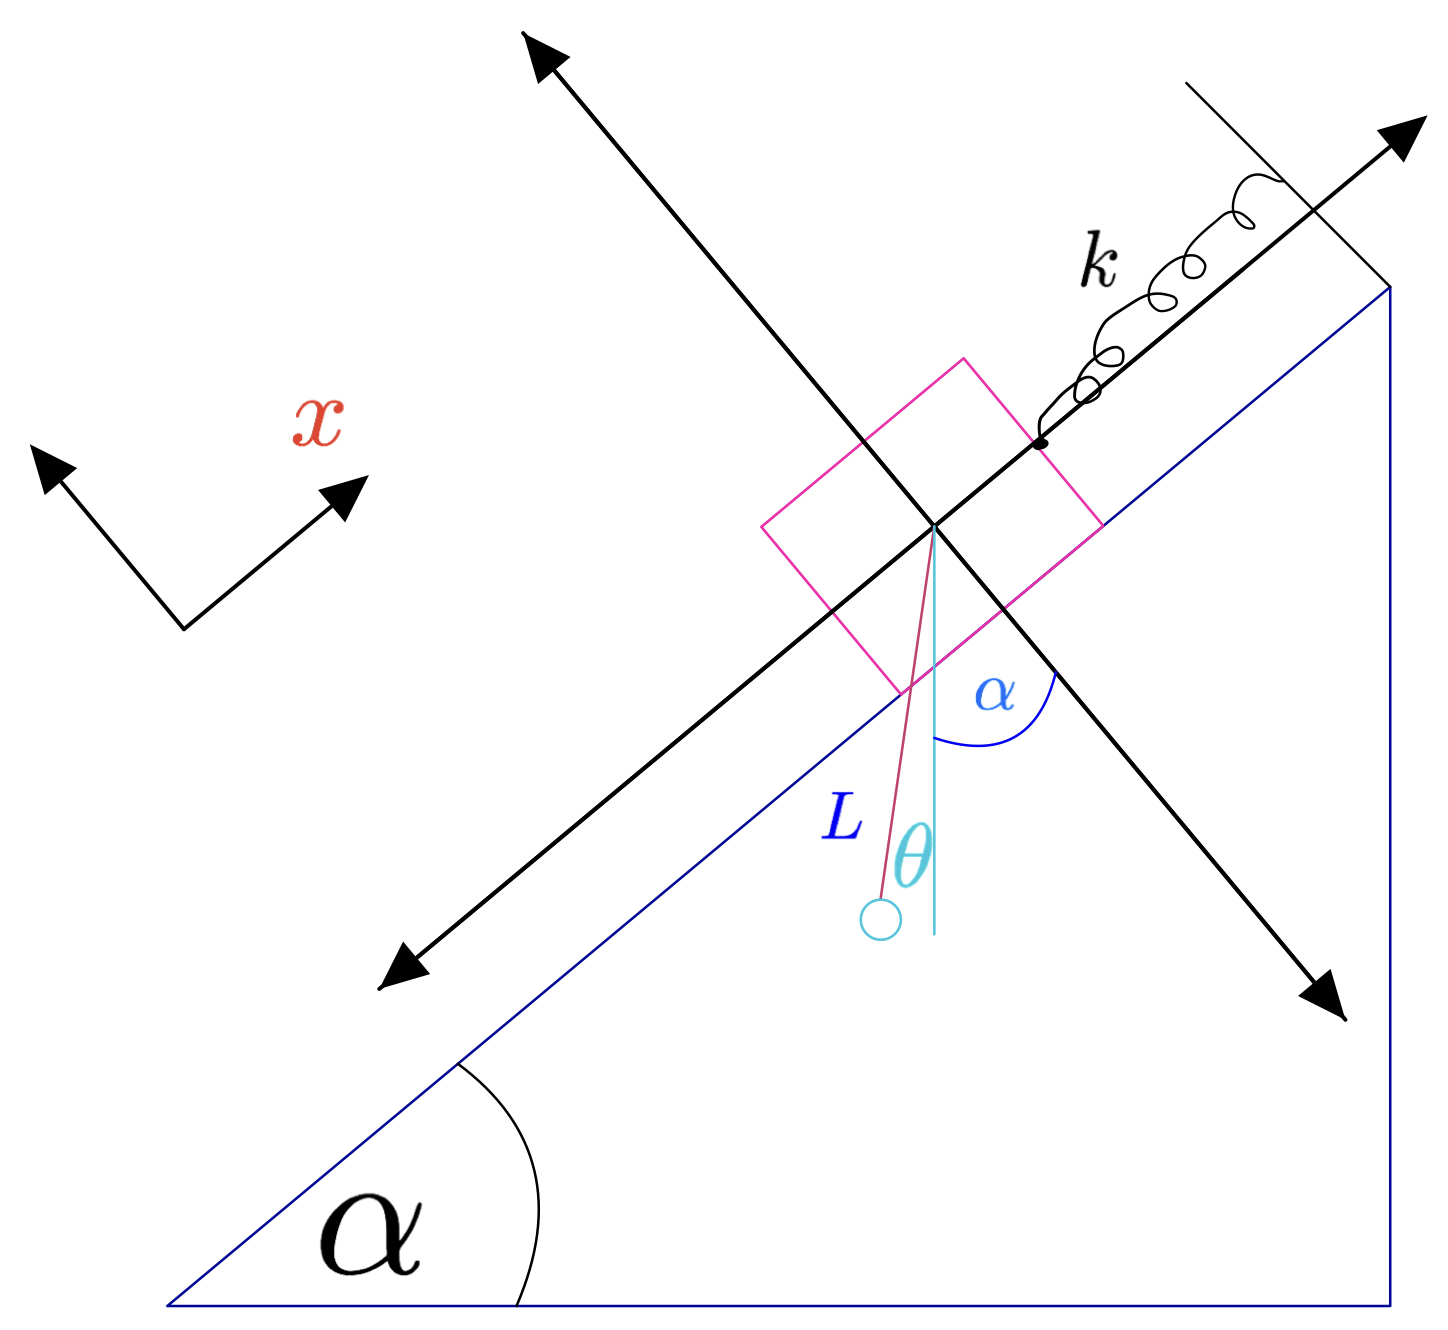
\includegraphics[width=0.5\textwidth]{dg_1.png}
    \caption{Diagrama de Problema 1 con Coordenadas x e L}
    \label{dg_1}
\end{figure}
Con lo cual si definimos las coordenadas generalizadas tenemos:
\begin{align}
(x,l):\,\,(x+L\sinn{\theta+\alpha},\,\,L-L\coss{\theta+\alpha})\\
(\dot{x},0):\,\, (\dot{x}+\dot{\theta}L\coss{\theta+\alpha},\,\, \dot{\theta}L\sinn{\theta+\alpha})	
\end{align}
Con esto la energía cinetica y potencial del sistema es:
\begin{align}
&T=\frac{1}{2}M \dot{x}^2 	+\frac{1}{2}m \qty(\dot{x}^2+L \dot{\theta}^2 +2\dot{x} \dot{\theta}L\coss{\theta+\alpha})\\
&U= MgL+mgL(1-\coss{\theta+\alpha})+\frac{1}{2}kx^2
\end{align}
Escribimos la energia cinetica en terminos de los momentos asociados a las coordenadas.
\begin{align}
	&T=\frac{1}{2M} p_x^2 	+\frac{1}{2m}\qty(p_{x}^2+L p_{\theta}^2 +2p_{x} p_{\theta}L\coss{\theta+\alpha})\\
	&U= MgL+mgL(1-\coss{\theta+\alpha})+\frac{1}{2}kx^2
\end{align}

Con esto si la coordenada $x \rightarrow q_1$ con $p_x  \rightarrpw p_1$ y $\theta \rightarrow q_2$ con $p_\theta \rightarrow p_2$ el Hamiltoniano del sistema es:

\en{\H= \frac{1}{2M} p_1^2 	+\frac{1}{2m}\qty(p_{1}^2+L p_{2}^2 +2p_{1} p_{2}L\coss{q_2+\alpha})+ MgL+mgL(1-\coss{q_2+\alpha})+\frac{1}{2}kq_1^2}
Ahora podemos obtener las ecuaciones de Hamilton correspondientes aplicando el corchete de Poisson al hamiltoniano tal como muestra el codigo ($ec1.nb$).
\begin{align}
&\boxed{\dot{q_1}=[q_1,\H]=	\frac{p1}{M}+ \frac{p_1+L p_2 \coss{q2+\alpha}}{m}\vl \dot{p_1}=-kq_1}\\
&\boxed{\dot{q_2}= \frac{Lp_2+ L p_1 \coss{q2+\alpha}}{m}\vl \dot{p_2}= -gLm\sinn{q_2+\alpha}+\frac{Lp_1 p_2 \sinn{q_2+\alpha}}{m}}
\end{align}
Podemos aproximar para pequeñas oscilaciones a primer orden las funciones trigonometricas, ya que nuestras coordenadas y momentos generalizados son pequeños.

\begin{align}
&\dot{q_1}=	\frac{p1}{M}+ \frac{p_1+L p_2 \qty(\coss{\alpha}-\sinn{\alpha}q_2)}{m}\vl \dot{p_1}=-kq_1\\
&\dot{q_2}= \frac{Lp_2+ L p_1 \qty(\coss{\alpha}-\sinn{\alpha}q_2)}{m}\vl \dot{p_2}= -gLm\qty(\sin{\alpha}+\coss{\alpha}q_2)+\frac{Lp_1 p_2 \qty(\sin{\alpha}+\coss{\alpha}q_2)}{m}
\end{align}
\s{Problema 2}
Se realizaron los corchetes de Poisson en el archivo ($ec1.nb$)de $[P1,Q1]$ obteniendo que esto vale $-\alpha \beta$ junto a esto se hicieron con  $[P2,Q2]$ obteniendo $-\alpha \beta $.Como estos deben valer -1 se tiene:\\
$$\alpha =  \beta \therefore \textit{Estos pueden valer por ejemplo: } \alpha = 1 \implies \beta = 1$$

Para armar la Generatriz podemos despejar $q_1$ y $q_2$ de sus Q's.
\begin{align}
q_2=Q_2 \coss{p_2}\\
q_1=\sqrt{Q_1}\\
\textit{Esto perfectamente puede ser una generatriz }F_3\\
q_2=Q_2 \coss{p_2}=-\pdv{F_3}{p_2}\\
q_1=\sqrt{Q_1}=-\pdv{F_3}{p_1}\\
\textit{Podemos reemplazar q1 y q2 en P1}\\
P_1= \frac{p_1 \coss{p_2} -2Q_2 \coss{p_2}}{2\sqrt{Q_1}p_2}=\frac{p_1 -2 Q_2}{2\sqrt{Q_1}}=-\pdv{F_3}{Q_1}\\
\textit{Se puede reemplazar q1 y q2 en P2 como se hizo antes}\\
P_2=\sinn{p_2}-2\sqrt{Q_1}=\pdv{F_3}{Q_2}
\end{align}

Ahora se puede hacer el metodo de variables separables e integrar la primera ecuacion, luego derivarla e igualarla a la siguiente para ir encontrando las constantes. Con esto tenemos que:
\begin{align}
F_3=-\sqrt{Q_1}p_1+h \bigg/ \pdv{p_2}\\
Q_2 \coss{p_2}=-\pdv{h}{p_2}\implies h= -Q_2 \sinn{p_2}+t\\
F_3=-\sqrt{Q_1}p_1 -Q_2 \sinn{p_2}+t\bigg/ \pdv{Q_1}\\
\frac{p_1}{2\sqrt{Q_1}} +\pdv{t}{Q_1}=p_1 \sinn{p_2} -2Q_2 \sinn{p_2}{2\sqrt{Q_1}p_2} \implies t=2\sqrt{Q_1}Q_2 + k\\
F_3=-\sqrt{Q_1}p_1 -Q_2 \sinn{p_2} + 2\sqrt{Q_1}Q_2 + k\bigg/ \pdv{Q_2}\\
\sinn{p_2}-2\sqrt{Q_1} +k'=\sinn{p_2}-2\sqrt{Q_1} \implies k=cte\\
\boxed{F=-\sqrt{Q_1}p_1 -Q_2 \sinn{p_2} + 2\sqrt{Q_1}Q_2 + C}
\end{align}

\end{document}